\documentclass[CS4402-Notes.tex]{subfiles}
\begin{document}

\section{Search}
\subsection{Definitions}
\subsubsection{Systematic search}
The idea of \textbf{search} is to make an educated guess among several available alternatives, but be prepared to undo the guess and try a different alternative if the guess does not lead to a solution. 
\n
More concretely, \textbf{systematic} search is the case where given sufficient time:
\begin{itemize}
\item If there is a solution, it will be found
\item If there is no solution, the search space will be exhausted and the search will report that there is no solution
\end{itemize}
Typically, search is done through \textbf{partial assignments} of one or more decision variables which begins with an empty assignment and incrementally attempts to extend it into a solution. In this context, a \textbf{backtracking} search is one where if it is discovered that the current partial assignment cannot be extended to a solution (a dead end), then the algorithm backtracks over the last decision made and tries and alternative assignment. 

\subsubsection{Tree traversal}
The search for a solution to a CSP can be easily viewed as exploring a tree where the root represents the CSP with no assigned variables and each choice corresponds to the branches of the tree. 
\begin{figure}[H]
\centering
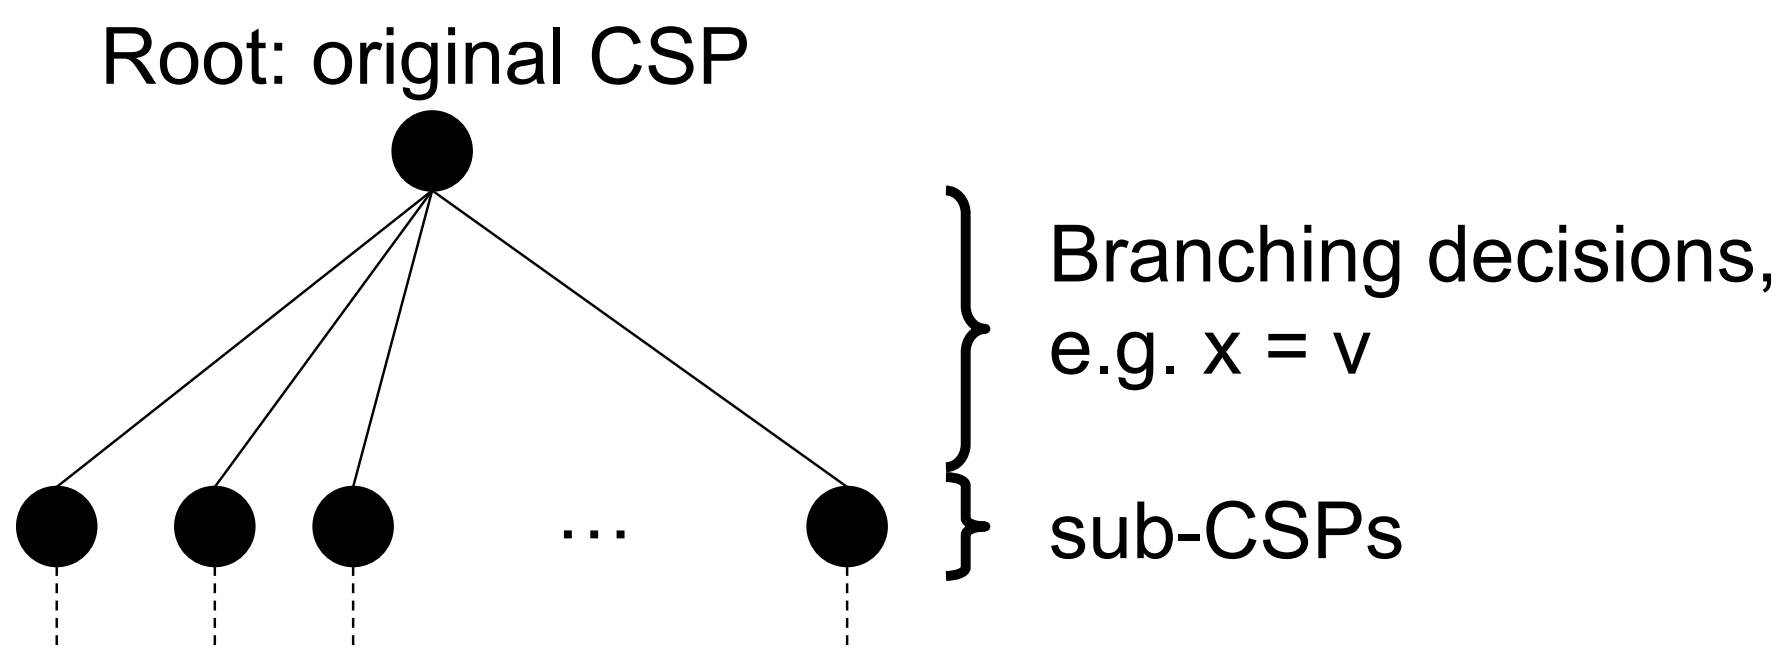
\includegraphics[width=0.85\textwidth, keepaspectratio]{imgs/csp-tree.png}
\caption{CSP search viewed as a tree.}
\end{figure}
\noindent
The descending nodes correspond to sub-CSPs which are the original CSP with partial assignments. Furthermore there are two common branching styles used for tree traversal: \textbf{d-way branching} and \textbf{2-way branching}.
\n
\textbf{D-way branching} \\
In d-way branching, each branch under the parent node represents the assignment of one of the $d$ domain values from the domain of a particular variable. For example, if $x \in \{1, 2, 3\}$, then there would be three branches which correspond to the assignment of $x$, one for each assignment. 
\n
\textbf{2-way branching} \\
\begin{figure}[H]
\centering
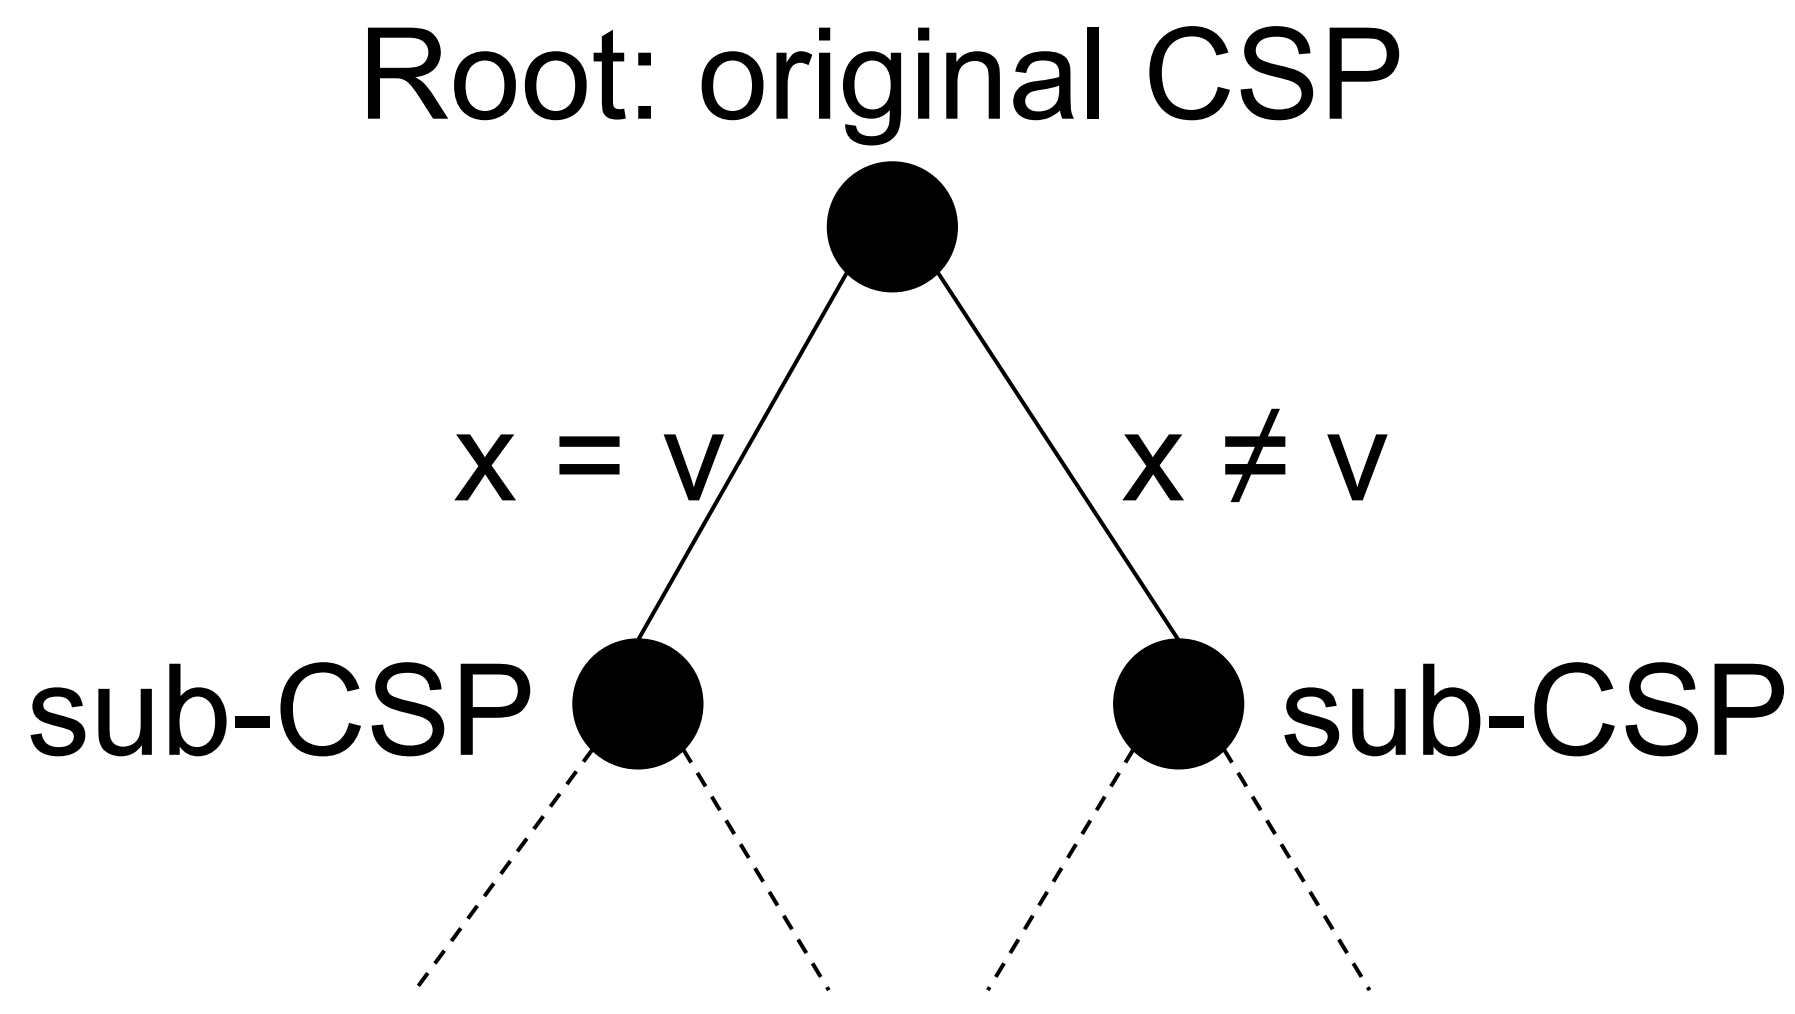
\includegraphics[width=0.4\textwidth, keepaspectratio]{imgs/2-way-branching.png}
\caption{2-way branching.}
\end{figure}
\noindent
In comparison, 2-way branching divides the search space into two pieces, one where the assignment to a particular domain value is true, and the other when it is false. The left branch tries to extend the partial assignment with $x = v$ first and if no solution is found down that branch, $v$ is removed from consideration entirely for the rest of the search. 

\subsubsection{Ordering}
In a search problem, there are both \textbf{variable orderings} and \textbf{value orderings}. They specify the order in which the variables are assigned and the order in which the values for the variables are tested. These can be either fixed or dynamic, depending on the heuristic. 
\n
Variables that have yet to be assigned are called \textbf{future} variables and similarly the variables that have been assigned are called \textbf{past} variables. 

\subsection{Methods}
\subsubsection{Generate and test}
Generate and test is a simple but very expensive method of solving a CSP. It is simply generating each \textbf{complete} assignment possible, then testing them all to see if any satisfy all the constraints. 
\n
This issue is further shown when trying to solve constraint \textit{optimisation} problems because simply satisfying the assignments is not enough it does not guarantee the best assignment. Therefore in this case, generate and test must examine all complete assignments except in the case where we know the current solution cannot be improved. 
\n
Simply put, generate and test is a brute force method that only checks constraints \textit{after} a complete assignment has been generated. It is systematic in that it is guaranteed to find a solution if one exists, however, due to its limitations in speed and memory it is never used in practice. 

\subsubsection{The backtrack algorithm}
The backtrack algorithm improves on generate and test by incrementally extending partial solutions. Every time an assignment is make, the constraints are checked to make sure none are violated. 
\subsubsection{Branch and bound}

\section{Propagation}


\end{document}
